\documentclass[14pt]{article}
%\documentclass[14pt]{llncs}
\usepackage[left=1.5cm,right=1.5cm,top=1.5cm,bottom=1.5cm]{geometry}
%\usepackage[a4paper, total={6in, 8in}]{geometry}
\usepackage{amsmath,amssymb,amsfonts} % mathematical and other 
% special symbols and fonts
\usepackage{tikz} % support for drawing graphs and diagrams
\usetikzlibrary{arrows,decorations.pathmorphing,positioning,fit}
\usetikzlibrary{trees,shapes}
\usepackage[pdfpagelabels=true,linktocpage]{hyperref} % hyperlink 
% support (also internal links)
\usepackage{xcolor} % color support
\usepackage{listings} % listings and \lstinline support for code 
% typesetting
\lstset{language=C++}
\usepackage[english]{babel} % needed for English texts (translations, 
% e.g. References --> Literatur)
% \usepackage[ngerman]{babel} % needed for German texts (translations, 
%e.g. References --> Literatur)
\usepackage[utf8]{inputenc} % unicode encoding
\usepackage{graphicx} % support for \includegraphics{}
\usepackage{float}
\usepackage{enumerate} % support of different styles of enumerations
%\usepackage[section]{algorithm}
\usepackage{newalg}
\usepackage{paralist}

\usepackage{url}
\usepackage{qtree}

\usepackage{tikz}
\usetikzlibrary{trees}

\usepackage{tikz}
\usetikzlibrary{shapes}
\usepackage{amsmath}
\usepackage{xspace}
\newcommand{\A}{\ensuremath{\mathcal{A}}\xspace}
\newcommand{\B}{\ensuremath{\mathcal{B}}\xspace}
\newcommand\pa[1]{\ensuremath{\left(#1\right)}}


\usepackage{dot2texi} 



\usepackage[listings,theorems]{tcolorbox}
\tcbset{before={\par\medskip\pagebreak[0]\noindent},after={\par\medskip}}%

\usepackage{amsmath}
\usepackage{booktabs}
\usepackage{caption}
\captionsetup[table]{position=top}


% By default the URLs are put in typewriter type in the body and the
% bibliography of the document when using the \url command.  If you are
% using many long URLs you may want to uncommennt the next line so they
% are typeset a little smaller.
\renewcommand{\UrlFont}{\small\tt}


\newtheorem{definition}{Definition}[section] % defines the definition environment
\newtheorem{theorem}{Theorem}[section] % defines the theorem environment
\newtheorem{proof}{Proof}[section] % defines the proof environment
\newtheorem{Algorithm}{Algorithm} % defines the algorithm environment

%\floatstyle{boxed}		% Puts a figure
%\restylefloat{figure}	% into a box.
\floatstyle{ruled}					% Puts an algorithm
\newfloat{Algorithm}{thp}{lop}		% between a head and
\floatname{Algorithm}{Algorithm}	% a foot line
\restylefloat{table}	% Puts a table between a head and a foot line



%Define often used expressions:
\newcommand{\True}{\ensuremath{\textit{True}~}}
\newcommand{\False}{\ensuremath{\textit{False}~}}
\newcommand{\TikZ}{Ti\emph{k}Z}

\newcommand{\rom}[1]{\uppercase\expandafter{\romannumeral #1\relax}}
%\renewcommand{\baselinestretch}{1.3}

% A nice opportunity to comment the text is given by the following:
%\usepackage{todonotes}
%\definecolor{lightgreen}{rgb}{0.8,1.0,0.8}
%\definecolor{lightblue}{rgb}{0.8,0.85,1}
%\newcommand{\Author}[1]{\todo[inline,color=lightgreen]{A: #1}}
%\newcommand{\Supervisor}[1]{\todo[inline,color=lightblue]{S: #1}}


\title{SMT for Strings \\ {\large Seminar:
		Satisfiability Checking} \\ {\large SS 2015}}
\author{Meshkatul Anwer \\ Supervision: Cornelius Aschermann}
%\institute{ RWTH Aachen}


\begin{document}
	
	\maketitle
	
    \begin{abstract}
Our modern society relies on software systems and on-line services. Most of the times these systems are dealing with our private and sensitive data. Privacy violation is one of the major concerns about such web-based applications and on-line services. To provide a more secure environment for the Internet services, these web-based applications should be tested for vulnerability. The verification procedure and security analysis of such system rely on automatic solvers, which can check the satisfiability of constraints over a rich set of data types, including character strings. String is considered as the main information carrier in web-based communication. However, most traditional mathematical methods focus more on numbers and most string solvers today are standalone tools that can reason only about some fragment of the theory of strings. In this paper we will describe a solver for the theory of unbounded strings with concatenation and length. 
\end{abstract}
	\section{Introduction}
\label{sec:introduction}
Stability and reliability of software systems has been a key issues in the protection of privacy and security. As we want more and more new features and functionalists into such systems, the complexity of the system is exploding. With the rise of web-based applications and online services, the amount of information sharing via networking has increased rapidly. As a result, the security of web applications is getting more and more attention. As the complexity of such systems is growing, manual analysis is getting harder and sometime impossible.  In the last few years, a number of techniques which were originally developed for automatic verification purposes have been adopted for the software security analysis. 

The ability to reason about string values is a major task in the field of security analysis. Especially in web-based applications, where the program inputs are often provided as strings. These strings are usually get processed through operations such as matching against regular expressions, concatenation, and substring extraction or replacement. We need to be able to formally reason about strings as well as other data types.  


In this paper, we will see how the automatic reasoning engines such as Satisfiability Module Theories (SMT) solvers, are helping to check the satisfiability of constraints over rich set of data types including  strings. We will describe a  SMT solver for strings. The ideas are presented in paper \cite{main-paper} and a practical version of the solver is implemented into the SMT solver CVC4 \cite{cvc4_website} core.
	\section{Motivating Example}
We are interested in SMT solver which helps to check the satisfiability of constraints over rich set of data types. Here we will see few examples such constraints on strings. Example 3 shows how we can express regular expression membership constraint.

\begin{description}
\item[Example  1: ] Find an assignment for \(x\), where \(x."ab"="ba".x \wedge  len(x) =7\).
\item[Example  2: ] Find a model for \(x\), \(y\) and \(z\), where \(x."ab".y=y."ba".z \wedge z=x.y \wedge x."a" \neq "a".x\).
\item[Example  3: ] Find a model for \(x\) and \(y\), where both \(x\) and \(y\) are in the \(RegEx (a*b)*\) and they are different but have the same length.
\end{description}
Where \(x\), \(y\) and \(z\) are variables of type string, \(len\) is a function which returns the length of the string variable.  Figure \ref{fig:smt_example_1_2} and \ref{fig:smt_example_3} show the encoding of Example 1 , Example 2 and Example 3 in smt-lib \cite{smtlib:website} format. The examples and code snippets  are taken from \cite{cvc4:wiki}.

\begin{figure}[ht]
	\centering
	\begin{minipage}[t]{0.45\linewidth}
		\begin{verbatim}
		...		
		(assert (= (str.++ x "ab") (str.++ "ba" x)))
		(assert (= (str.len x) 7))
		
		...
		\end{verbatim}
	\end{minipage}
	\quad
	\begin{minipage}[t]{0.45\linewidth}
		\begin{verbatim}
		...
		(assert (= (str.++ x "ab" y) (str.++ y "ba" z)))
		(assert (= z (str.++ x y)))
		(assert (not (= (str.++ x "a") (str.++ "a" x))))
		...
		\end{verbatim}
	\end{minipage}
	\caption{Encoding of Example 1 and Example 2 in smt-lib \cite{smtlib:website} format.}
	\label{fig:smt_example_1_2}
\end{figure}
\begin{figure}[ht]
	\centering
    \begin{minipage}[t]{0.65\linewidth}
		\begin{verbatim}
		...
		(assert(str.in.re x(re.* (re.++ (re.* (str.to.re "a") ) (str.to.re "b") ))))
		(assert (str.in.re y(re.* (re.++ (re.* (str.to.re "a") ) (str.to.re "b") ))))
		
		(assert (not (= x y)))
		(assert (= (str.len x) (str.len y)))
		...
		\end{verbatim}
	\end{minipage}
	\caption{Encoding of Example 3 in smt-lib \cite{smtlib:website} format.}
	\label{fig:smt_example_3}
\end{figure}

In the context of security analysis, modern SMT solver is used as the core constraint solver. The idea is to reduce security problems to constraint satisfaction problems in some formal logic. If the constraints are unsatisfiable, the source code is free of any exploit; otherwise, there is an assignment (of variables in the constraints) that satisfies these constraints and defines a possible attack. Traditionally analysis tools use their own built-in constraint solvers. However, it is possible to encode a security analysis problem into a Satisfiability Modulo Theories (SMT) problem. Then the preexisting standard SMT solver, which combines a SAT solver with multiple specialized theory solvers can be used. As string is the dominant data type in modern web-applications, constraints over strings along with other data types need to be checked. In this paper we will have a look into a string solver.
	
	\section{Related work}
\label{sec:Related work}

There has been a lot of research effort on the development of the efficient theory solver for Strings \cite{misc_89}. Theoretically the general world equation problem or the satisfiability problem of theory of strings(with most of common string functions) is undecidable \cite{misc_17}. However, a restricted theories of strings is decidable and practically useful. Different approaches to solve the problem have been proposed and implemented. A class of solvers is based on reducing the string constraints to constraints in other theories e.g. theory of bit-vector. Examples of such solver are Hampi \cite{hampi} and Kaluza \cite{Kaluza}. However, they can only solve problem over fixed length strings. 

In this paper, we will present a SMT solver for strings based an algebraic approach. The whole decision procedure is described as a set of derivation rules and their application strategy. The procedure allows to express the constraints over unbounded strings. A practical theory solver over string based on this approach has been implemented into the CVC4 SMT solver\cite{cvc4_website} core. The detail of the description can be found in the paper \cite{main-paper}. We will try to explain the main ideas presented by the authors.    
	
\section{Preliminaries}
\label{sec:Preliminaries}
In this section, we will present an introduction over the DPLL($\mathcal{T}$) procedure and architecture. The reader can skip this section, if the concepts are clear to them. In the subsequent sections we will present a formal description of the theory solver as a set of normalization rewrite rules, derivation rules and a proof procedure.

\subsection{The DPLL($\mathcal{T}$) Procedure}
\label{sec:dpllt procedure}
In propositional logic, a formula is constructed from a set of boolean variables using a set of logical connectives, such as \(\wedge, \vee, \neg\). Boolean variables can be assigned a truth value that is either  $\texttt{true}$ or  $\texttt{false}$. Given a Boolean formula, the boolean satisfiability problem (SAT) is to answer whether there is an assignment for those variables, such that the formula is evaluated to be $\texttt{true}$. There are many decision procedures to solve the classic SAT problem. Among them, the DPLL procedure is the most frequently used in most modern SAT solvers. 

The DPLL procedure takes a set of clauses as input. It returns $\texttt{sat}$ if a logically consistent assignment can be found; otherwise, it returns $\texttt{unsat}$. During its computation, the procedure maintains an internal stack of literals (possibly with decision marks) to represent a partial assignment. 

Whenever every clause is evaluated to be $\texttt{true}$ under the current assignment, the procedure stops and returns $\texttt{sat}$. During a standard processing loop, the DPLL procedure processes the clause set in three steps:

\begin{description}
	\item[1] It first checks whether the current partial assignment is consistent with the clause set by evaluation. If one of the clauses is evaluated to $\texttt{true}$ and the stack contains at least one decision literal, the procedure pops out all literals in the stack till the nearest decision literal, then flips the sign of that decision literal and turns it into a propagation literal. This step is often referred to \(backtrack\). If one of the clauses is evaluated to $\texttt{false}$ and the stack does not contain one decision literal, the procedure stops and returns $\texttt{unsat}$.
	
	\item[2] After the inconsistent check, the procedure tries to push new propagation literals into the stack by logical deduction. This is known as Unit Propagation.
	
	\item[3] If there are still unassigned variables, the procedure picks one heuristically, guesses its sign, and pushes it into the stack as a decision literal.
\end{description}

The procedure continues until all variables are assigned. In our context, the SAT solver should be able to handle incremental clause assertions. 

\begin{figure}[htb]
	\begin{center}
		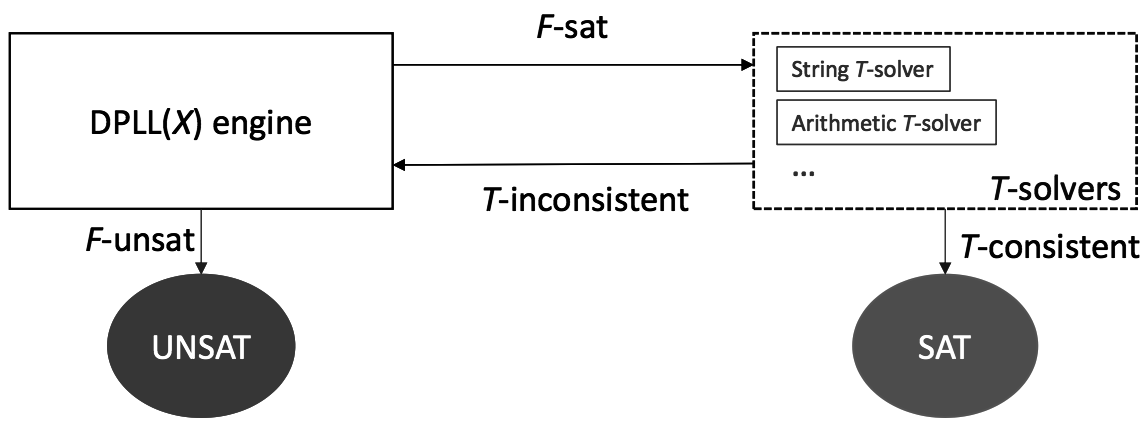
\includegraphics[width=0.8\linewidth]{pictures/dpll_arc.png}
	\end{center}
	\caption{A general DPLL(\(T\)) Architecture. The image is taken from \cite{main_phd}.}
	\label{fig:dpll_architecture}
\end{figure}

\subsection{The DPLL($\mathcal{T}$) Architecture}
\label{sec:The DPLL(T) Architecture}
In Boolean formulas, the signature only contains propositional variables and logical connectives.But in SMT formulas, the signature is extended to a set of predicate symbols, a set of function symbols and a set of non-boolean variables. Those extended symbols can be interpreted in some background theories. An SMT formula is satisfiable if there exists a model that satisfies both the logical formula and the background theories.

Reasoning about an SMT formula usually involves several reasoning over several theories. We refer the procedure to reason over a theory $\mathcal{T}$ as a $\mathcal{T}$-solver. Note that a $\mathcal{T}$-solver can only handle conjunctions of literals. Given a formula over several theories where each theory has a $\mathcal{T}$-solver, the Nelson-Oppen combination \cite{nelson_oppen} provides a procedure to reason about this constraint.

The DPLL($\mathcal{T}$) architecture can be divided into two parts, as shown in Figure \ref{fig:dpll_architecture} : the logic solving part and the theory solving part. In the logic solving part, it usually refers to the DPLL-based SAT solver with  the capability to handle incremental clause assertions. 

The theory solving part usually contains several dedicated solvers for background theories, called $\mathcal{T}$-solvers. Compared to a generic theory solver, a $\mathcal{T}$-solver requires the mechanisms for incrementality and backtracking. A $\mathcal{T}$-solver maintains a set of $\mathcal{T}$-related literals. This set is a subset of the partial assignment $\mathcal{M}$.

Initially, the SAT solver gets the formula $\mathcal{F}$ from the input. It tries to find a model for the literals. If failed, it returns $\texttt{unsat}$; otherwise, it distributes each literal in $\mathcal{M}$ to a corresponding $\mathcal{T}$-solver according to some $\mathcal{T}$-signature-based heuristics.

When a $\mathcal{T}$-solver gets a set of literals, it first checks whether these literals are consistent with the theory. If it is $\mathcal{T}$-consistent, the $\mathcal{T}$-solver does nothing but reports consistent back to the main engine. If it is $\mathcal{M}$-inconsistent, it either returns a conflict (in a form of literal conjunction), or propagates a new literal with an explanation (in a form of implication).

If all $\mathcal{T}$-solvers report $\mathcal{T}$-consistent, the procedure stops and answers $\texttt{sat}$ with the model $\mathcal{M}$; otherwise, the SAT solver collects all clauses returned by $\mathcal{T}$-solvers, and asserts them into the formula $\mathcal{F}$. Then, it tries to build a model from this new formula.

	

	%\section{A Theory of Strings and Regular Language Membership}
\label{sec:Theories over Strings}
We use \textbf{Str}, \textbf{Lan} and \textbf{Int} to denote the String sort, the Language sort and the Integer sort, respectively. We use \( \Sigma_{SRL_p}\) to denote the signature with three sorts \textbf{Str}, \textbf{Lan} and \textbf{Int}. \(\mathcal{T}_{SRL_p}\) refers to the theory of strings with length and positive regular language membership constraints over a signature \( \Sigma_{SRL_p}\). The interpretations of \(\mathcal{T}_{SRL_p}\) differ only on the variables. They all interpret \textbf{Int} as the set of integer numbers  \(\mathbb{Z}\), \textbf{Str} as the set of all strings  \(\mathbb{S}\)  over some fixed finite alphabet  \(\mathcal{A}\) of characters, and \textbf{Lan} as the power set of \(\mathcal{A}^* \).
The signature includes the following predicate and function symbols:
The common symbols (e.g., \( + , - ,  \le \) ) of linear integer arithmetic are interpreted as usual. The signature of the sort \textbf{Str} consists the following symbols:

\begin{description}
	\item[-] a constant symbol, or string constant, for each word of \(\mathcal{A}^* \), interpreted as word;
	\item[-] a function symbol \($\underline{con}$ : String \times \cdots \times String \to String\), interpreted as the word concatenation;
	\item[-] a function symbol \($\underline{len}$ : String  \to Int \), interpreted as the word length function;    
\end{description}
The signature of the sort  \textbf{Lan} consists the following symbols:
\begin{description}
	\item[-] a function symbol \($\underline{set}$ : String  \to Lan \), interpreted as the function mapping each word  \( w \in \mathcal{A}^* \) to the language  \(\{w\}\);
	\item[-] a function symbol \($\underline{star}$ : Lan \to Lan\), interpreted as the Kleene clousre operator;
	\item[-] a predicate symbol \($\underline{in}$ : String \to Lan\), interpreted as the membership predicate;	
	\item[-] a suitable set of additional function symbols: \(union, inter, rempty, allchars, opt range, loop, plus, comp \), interpreted as language concatenation, conjunction and so on;
\end{description}
We define three types of terms:
\begin{description}
	\item[-] \( string \ term \) : any term of sort \textbf{Str} or of the form \((len \ x )\);
	\item[-] \( arithmetic \ term \) : any term of sort \textbf{Int} all of whose occurrences of \(len\) are applied to a variable;
    \item[-] \( regular \ expression \) : any term of sort \textbf{Lan}(possibly with variables).
\end{description}
A \( string \ term \) is \( atomic \) if it is a variable or a string constant. We define three types of constraints:
\begin{description}
	\item[-] \( string \ constraint \) : is a (dis)equality  \( (\neg) s \approx t \) with \(s\) and \(t\) are string terms;
	\item[-] \( arithmetic \ constraint \) : is a (dis)equality  \( (\neg) s \approx t \) or \( (\neg) s > t \) where \(s\) and \(t\) are arithmetic terms;
	\item[-] \( RL \ constraint \) : is a literal of the form \((s \textnormal{in} r)\) where \(s\) is a string term and \(r\) is a regular expression.
\end{description}

Note that if \(x\) and \(y\) are string variables, \(\textnormal{len} \ x\) is both a string and an arithmetic term and  \((\neg)\textnormal{len} \ x \approx \textnormal{len} \ y\) is both a string and an arithmetic constraint. A \(\mathcal{T}_{SRL_p}\)-constraint is a string, arithmetic or RL constraint. We will use \( \models_{SRL_{p}}\) to denote entailment in \(\mathcal{T}_{SRL_p}\).
    \section{The Theory solver $ \mathcal{T}_{SL}$}
\label{sec:the theory solver}
\subsection{Objective }
\label{sec:objective}
We want a solver to handle a finite set of (unbounded)string constraints, length constraints and regular language memberships. Most of the other solvers available in the market try to solve the constraints by converting them into constraints of other available theories. Here we will see, the algebraic approach taken by the authors of cvc4 \cite{cvc4_website} to implement the solver. The solver is described as a rule-based procedure by the original authors in \cite{main-paper}. Before we go into detail, we will present few formal preliminaries and definitions. We will focus our discussion only on solving string constraints and length constraints.

\subsection{Basic}
\label{sec:basic}
A $theory$ is a pair $\mathcal{T} = (\Sigma\ \texttt{I})$ where $\Sigma$ is a signature and \texttt{I} is a class of $\Sigma$-interpretations, that is closed under variable reassignment. A $\Sigma$-formula $\varphi$ is $satisfiable$ (resp., $unsatisfiable$) in $\mathcal{T}$ if it is satisfied by some interpretation in \texttt{I}. A set $\Gamma$ of formulas entails in $\mathcal{T}$ a $\Sigma$-formula $\varphi$, written $\Gamma \models_{T} \varphi$ , if every interpretation in \texttt{I} that satisfies all formulas in $\Gamma$ satisfies $\varphi$ as well. The set $\Gamma$ is $satisfiable$ in $T$ if $\Gamma \models_{T} \perp$ where $\perp$ is the universally false atom. We will write $ \Gamma \models \varphi$ to denote that $ \Gamma$ entails $\varphi$ in the class of all $\Sigma$-interpretations. We will use $\approx$ as the (infix) logical symbol for equality, which has type $\sigma \times \sigma$ for all sorts $\sigma$ in $\Sigma$ and is always interpreted as the identity relation. We write $s \not\approx t$ as an abbreviation of $\neg s \approx t$. These notations are defined by the original authors in \cite{main-paper} and we will also use them with the same context in the subsequent sections.


\subsection{Core language}
\label{sec:Theories over Strings}
We use \textbf{Str}, \textbf{Lan} and \textbf{Int} to denote the String sort, the Language sort and the Integer sort, respectively. We use \( \Sigma_{SRL_p}\) to denote the signature with three sorts \textbf{Str}, \textbf{Lan} and \textbf{Int}. \(\mathcal{T}_{SRL_p}\) refers to the theory of strings with length and positive regular language membership constraints over a signature \( \Sigma_{SRL_p}\). The interpretations of \(\mathcal{T}_{SRL_p}\) differ only on the variables. They all interpret \textbf{Int} as the set of integer numbers  \(\mathbb{Z}\), \textbf{Str} as the set of all strings  \(\mathbb{S}\)  over some fixed finite alphabet  \(\mathcal{A}\) of characters, and \textbf{Lan} as the power set of \(\mathcal{A}^* \).
The signature includes the following predicate and function symbols:
The common symbols (e.g., \( + , - ,  \le \) ) of linear integer arithmetic are interpreted as usual. The signature of the sort \textbf{Str} consists the following symbols:

\begin{description}
	\item[-] a constant symbol, or string constant, for each word of \(\mathcal{A}^* \), interpreted as word;
	\item[-] a function symbol \($\underline{con}$ : String \times \cdots \times String \to String\), interpreted as the word concatenation;
	\item[-] a function symbol \($\underline{len}$ : String  \to Int \), interpreted as the word length function;    
\end{description}
The signature of the sort  \textbf{Lan} consists the following symbols:
\begin{description}
	\item[-] a function symbol \($\underline{set}$ : String  \to Lan \), interpreted as the function mapping each word  \( w \in \mathcal{A}^* \) to the language  \(\{w\}\);
	\item[-] a function symbol \($\underline{star}$ : Lan \to Lan\), interpreted as the Kleene clousre operator;
	\item[-] a predicate symbol \($\underline{in}$ : String \to Lan\), interpreted as the membership predicate;	
	\item[-] a suitable set of additional function symbols: \(union, inter, rempty, allchars, opt range, loop, plus, comp \), interpreted as language concatenation, conjunction and so on;
\end{description}
We define three types of terms:
\begin{description}
	\item[-] \( string \ term \) : any term of sort \textbf{Str} or of the form \((len \ x )\);
	\item[-] \( arithmetic \ term \) : any term of sort \textbf{Int} all of whose occurrences of \(len\) are applied to a variable;
	\item[-] \( regular \ expression \) : any term of sort \textbf{Lan}(possibly with variables).
\end{description}
A \( string \ term \) is \( atomic \) if it is a variable or a string constant. We define three types of constraints:
\begin{description}
	\item[-] \( string \ constraint \) : is a (dis)equality  \( (\neg) s \approx t \) with \(s\) and \(t\) are string terms;
	\item[-] \( arithmetic \ constraint \) : is a (dis)equality  \( (\neg) s \approx t \) or \( (\neg) s > t \) where \(s\) and \(t\) are arithmetic terms;
	\item[-] \( RL \ constraint \) : is a literal of the form \((s \ \textnormal{in} \ r)\) where \(s\) is a string term and \(r\) is a regular expression.
\end{description}

\subsection{The foundation}
We have a finite set of constraints of type string constraints and arithmetic constraints. The string solver takes this set as input and checks for satisfiability. If it finds a satisfying solution, it reports the set of constraints is satisfiable otherwise reports as \texttt{unsat}. From now on we will only consider string constraints and arithmetic constraints. If \(x\) and \(y\) are string variables, \(\texttt{len} \ x\) is both a string and an arithmetic term and  \((\neg)\texttt{len} \ x \approx \texttt{len} \ y\) is both a string and an arithmetic constraint. A \(\mathcal{T}_{SL}\)-constraint is a string, arithmetic constraint. We will use \( \models_{SL}\) to denote entailment in \(\mathcal{T}_{SL}\). Now we will present few definitions, which are defined by author in \cite{main-paper}. These definitions are used for the detail description of the decision procedure.


\begin{definition}{congruence closure of \(S\)}
\end{definition}
	Let \(S\) be a set of string constraints and let \( \mathcal{T}(S)\) be the set of all terms (and subterms) occurring in \(S\). The \(congruence \ closure\) of \(S\) is the set 
	\begin{gather*}
	\mathcal{C}(S) = \{  s\approx t | s, t \in \mathcal{T}(S), S \models s \approx t\} \cup
			\{ l_1 \not\approx l_2 \ \textnormal{distinct string cons.}\}   \cup \\ \{  s \not\approx t | s, t \in \mathcal{T}(S), s' \not\approx t' \in S, S \models s \approx s' \wedge t \approx t' \ \ \textnormal{for some.} s', t' \}
	\end{gather*}
	This equation is taken from \cite{main-paper}.	
	
	
\begin{definition}{equivalence relation}
\end{definition}
Iff \( s \approx t \in \mathcal{C}(S)\), where $ s, t \in \mathcal{T}(S) $, the terms \(s, t\) are called $equivalent$. For all \(t \in \mathcal{T}(\textnormal{S})\), its equivalence class in \( \textnormal{E}_S \) is denoted by \( [t]_S \). Where  \( \textnormal{E}_S \) is an $equivalence \ relation$ over \( \mathcal{T}(S) \) induced by the constraints in \(S\).

\begin{definition}{normalized form}
\end{definition}
A term is in $normalized \ form$, if it can not be reduced any more respect to the rewrite rules. The rewrite rules are shown in Figure \ref{fig:normalization_rewrite_rules}. For example, $(x, \epsilon, c_1, c_2c_3, y)$ becomes $(x, c_1c_2c_3, y)$ after the reduction.
\begin{figure}[htb]
\begin{minipage}{.45\linewidth}
\[
 \texttt{con}(\mathbf{s},  \texttt{con}(\mathbf{t}), \mathbf{u}) \rightarrow   \texttt{con}(\mathbf{s}, \mathbf{t}, \mathbf{u})
\]
\[
\texttt{con}(\mathbf{s}, \epsilon, \mathbf{u}) \rightarrow \texttt{con}(\mathbf{s}, \mathbf{u})
\]
\[
 \texttt{con}(s) \rightarrow s
\]
\[
 \texttt{con}() \rightarrow \epsilon
\]
\end{minipage}%
\begin{minipage}{.45\linewidth}
\[
 \texttt{con}(\mathbf{s}, c_1 \cdots c_i, c_{i+1} \cdots c_n, \mathbf{u}) \rightarrow \texttt{con}(\mathbf{s}, c_1 \cdots c_n, \mathbf{u})
\]
\[
 \texttt{len}( \texttt{con}(s_1,\cdots,s_n)) \rightarrow \texttt{len}(s_1) + \cdots + \texttt{len}(s_n)
\]
\[
  \texttt{len}(c_1,\cdots,c_n) \rightarrow n
\]
\end{minipage}
\caption{Normalization rewrite rules for terms. The rules are taken from \cite{main-paper}}
\label{fig:normalization_rewrite_rules}
\end{figure}

\begin{definition}{configurations}
\end{definition}
 A \(configuration\) is defined in \cite{main-paper} as a tuple of the form \( \langle \textnormal{S, A, R, F, N, C, B} \rangle \) where	
	\begin{description}	
		\item[-] S, A, R are respectively a set of string, arithmetic, and RL constraints;
		\item[-] F is a set of pairs $ s \mapsto \mathbf{a} $ where $ s \in \mathcal{T}(\textnormal{S})$ and $\mathbf{a}$ is a tuple of atomic string terms;
		\item[-] N is a set of pairs $ e \mapsto \mathbf{a} $ where $e$  is an equivalence class of \( \textnormal{E}_S \) and $\mathbf{a}$ is a tuple of atomic string terms;
		\item[-] C is a set if terms of sort \textbf{Str};
		\item[-] B is a set of $buckets$ where each bucket is a set of equivalence classes of \( \textnormal{E}_S \). For each bucket $ B \in \textnormal{B}, len_B$ denotes a unique term $\texttt{len}\ x$, where $[x] \in B.$
	\end{description}
	Initially the sets S, A, R store the input problem and grow with the introduction of new constraints derived by derivation rules. C stores terms whose flat form should not be computed, to prevent loops in the computation of their equivalence class normal form. B eventually becomes a partition of \( \textnormal{E}_S \). The procedure assigns string constants of different lengths to variables in different buckets, and different string constants of the $same$ length to different variables in the same bucket.
	
	A configuration is called $saturated$ by author in \cite{main-paper}, if
    \begin{itemize}
	   	\item \texttt{N} is a total map over \( \textnormal{E}_S \).
	   	\item \texttt{B} is a partition of \( \textnormal{E}_S \), and
	   	\item It is not possible to apply any derivation rule on the terms other than \texttt{Reset}.
	\end{itemize}
	The decision procedure concludes $\texttt{sat}$ when it reaches such a configuration in the derivation tree.
	
\begin{definition}{derivation rule}
\end{definition}
A $derivation rule$ applies to a $configuration\ K$, if all of the rule's premises hold. A rule's conclusion describes how each component of the $configuration\ K$ is changed, if at all. An application of rule may produce two or more beaches in the derivation tree. These rules have the symbol $\parallel$ in their conclusion. The author in \cite{main-paper} called them as are non-deterministic branching rules.
However, in the implementation the branching is applied from left to write. According to the author the derivation rules are only applicable on any configuration when it maintain the following conditions as $Invariant$:
\begin{description}			
\item[-] All terms are reduced with respect to the rewrite system in Figure \ref{fig:normalization_rewrite_rules}.
\item[-] \texttt{S} is a partial map from  $\mathcal{T}(\texttt{S})$ to normalized tuples of atomic terms.
\item[-] \texttt{S} is a partial map from \( \textnormal{E}_S \) to normalized tuples of atomic terms.
\item[-] For all terms $s$ where $[s] \to (a_1,\cdots,a_n) \in N$ or $s \to (a–1,\cdots,a_n) \in F$, we have $S \models_{SLR_p} \  s \approx \texttt{con}(a_1,\cdots,a_n)$ and $S \models a_i \not\approx \epsilon for i = 1,\cdots,n $.
\item[-] For all $B_1, B_2 \in \texttt{B}, [s] \in B_1$ and $[t] \in B_2, S \models \texttt{len} \ s \approx \texttt{len} \ t$ iff $B_1 = B_2$.
\item[-] \texttt{C} contains only reduced terms of the form $\texttt{con}(\mathbf{a})$.       	       
\end{description}
 
    In the paper \cite{main-paper} the authors have presented a list of the derivations rules. These rules are listed in Figures from \ref{rules_1} to \ref{rules_5}. Due to space restriction, we will only describe few of them bellow. 
    
    The first four rules $\texttt{A-Prop},\texttt{S-Prop},\texttt{Len}$ and $\texttt{Len-Splite}$  in Figure \ref{rules_1} describe the interaction between arithmetic solver and string solver. This is achieved via the propagation of entailed constraints on the shared terms. The rule $\texttt{A-Conflict}$ derives \texttt{unsat} if the arithmetic part of the constraints unsatisfiable. The basic rules for string constraints e.g. $\texttt{S-Cycle},\texttt{S-Split},\texttt{S-Conflict}$ are shown in Figure \ref{rules_2}. The functionality of \texttt{S-Split}, \texttt{L-Split} is straightforward. \texttt{S-Conflict} derives  \texttt{unsat} if $\mathcal{C}(S)$ contains both equality and dis-equality between the same pair of strings. \texttt{S- Split}  tries to guess whether two strings are equal or not, while \texttt{L-Split} tries to guess whether two string variables have the same length.  Application of split rules causes the branching of the derivation tree. \texttt{Reset} is meant to be applied when new constraints are introduced to the set $S$. The major part of the work is done by the $normalization\ derivation\ rules$ and $equality\ reduction\ rules$. These rules shown in Figures \ref{rules_3} and \ref{rules_4}. Detail about the individual rule can be found in \cite{main_phd} and in \cite{main-paper}.
   
   
   
   \begin{figure}
\scriptsize
\begin{minipage}{1.0\textwidth}
\begin{gather*}\label{eA1}
 \texttt{A-Prop} \frac{ S \models  \texttt{len} \ x \approx \texttt{len} \ y}{ A := A, \texttt{len} \ x \approx \texttt{len} \ y}\\
  \texttt{S-Prop} \frac{ A \models_{LIA}  \texttt{len} \ x \approx \texttt{len} \ y}{ S := S, \texttt{len} \ x \approx \texttt{len} \ y}\\
 \texttt{Len} \frac{ x \approx t \in \mathcal{C}(S) \ x \in \mathcal{V}(S)}{ A := A, \texttt{len} \ x \approx (\texttt{len} \ t) \downarrow}\\
 \texttt{Len-Split} \frac{ x \in \mathcal{V}(S \cup A) \ x: Str}{ S := S, x \approx \epsilon \parallel  A:= A, \texttt{len} \ x > 0}\\
 \texttt{A-Conflict} \frac{ A \models_{LIA} \perp }{ \texttt{unsat}}\\
 \texttt{R-Star} \frac{ s \ in \ star( set \ t) \in R \ s  \not\approx \epsilon \in \mathcal{C}(S)}{ S:= S, s \approx \textnormal{con}(t,z) \textnormal{R}:= \textnormal{R}, z \ in \ star \ (set \ t)}
\end{gather*}
\end{minipage}
\caption{ The rules for theory combination\cite{main-paper}. \texttt{R-Start} is handle cases with regular expression. }
\label{rules_1}
\end{figure}
   \begin{figure}
\begin{minipage}{1.0\textwidth}
\scriptsize
\begin{gather*}\label{eA1}
 \texttt{S-Cycle} \frac
 { t = \texttt{con}(t_1, \cdots, t_i, \cdots, t_n) \ t \in \mathcal{T}(S) \setminus C \ t_k \approx \epsilon \in \mathcal{C}(S) \ \textnormal{for all} \ k \in \{1,\cdots,n\} \setminus \{ i \} }
 { S := S, t \approx t_i \ C:=C (C, t) \setminus \{t_i\}   }\\
  \texttt{Reset} \frac{ }
  { \textnormal{F} := \phi, \textnormal{N} := \phi, \textnormal{B} := \phi}\\
   \texttt{S-Split} \frac
   { x, y \in \mathcal{V}(S) \ \ x \approx y, x \not\approx y \in \mathcal{C}(S) }
   { S := S, x \approx y \parallel S:= S, x \not\approx y}\\
      \texttt{S-Conflict} \frac
      { x \approx t \in \mathcal{C}(S) \ \ s \not\approx t \in \mathcal{C}(S)}
      { \textnormal{unsat}}\\
      \texttt{L-Split} \frac
       { x, y \in \mathcal{V}(S) \ \ x,y: \textnormal{Str}  \ \  S \not\models \texttt{len} \ x \not\approx \texttt{len} \ y}
       { S:= S, \texttt{len} \ x \approx \texttt{len} \ y \parallel S:=S, \texttt{len} \ x \not\approx \texttt{len} \ y}
\end{gather*}
\end{minipage}
\caption{Basic string derivation rules \cite{main-paper}.}
\label{rules_2}
\end{figure}

   \begin{figure}
\begin{minipage}{1.0\textwidth}
\scriptsize
\begin{gather*}\label{eA1}
 \bold{F-Form1} \frac
 { t = \textnormal{con}(t_1, \cdots,t_n) \ t \in \mathcal{T}(S) \setminus ( \mathcal{D}(F) \cup C)  \ \  N[t_1] = s_1 \cdots N[t_n] = s_n }
 { \textnormal{F} := \textnormal{F}, t \mapsto ( s_1, \cdots, s_n) \downarrow}\\
 \bold{F-Form2} \frac
 { l \in \mathcal{T}(S) \setminus \mathcal{D}(F)}
 { \textnormal{F} := \textnormal{F}, t \mapsto ( l)} \\
  \bold{N-Form1} \frac
  { [x] \not\in \mathcal{D}(N) \ \ s \in [x] \setminus ( C \cup \mathcal{V}(S)) \ \ F t= F s \textnormal{for all} \ t \in [x] \setminus ( C \cup \mathcal{V}(S)) }
  { \textnormal{N}:= \textnormal{N}, [x] \mapsto F s}\\
  \bold{N-Form2} \frac
  { [x] \not\in \mathcal{D}(N) \ \ [x] \subseteq  C \cup \mathcal{V}(S)} 
  { \textnormal{N}:= \textnormal{N}, [x] \mapsto (x)}
\end{gather*}
\null
\par\xdef\tpd{\the\prevdepth}
\end{minipage}
\caption{Normalization derivation rules. The letter \(l\) denotes a string constant.The rules are taken from \cite{main-paper} and they are in their original form.}
\label{rules_3}
\end{figure}
   \begin{figure}
\begin{minipage}{1.0\textwidth}
\scriptsize
\begin{gather*}\label{eA1}
 \texttt{F-Unify} \frac
 { F \ s = ( w,u,u_1) \ \ F \ t = (w, u,v_1)  s\approx t \in \mathcal{C}(S) \ S \models \texttt{len} \ u \approx \texttt{len} \ v }
 { S:= S, u \approx v}\\
  \texttt{F-Split} \frac
  {\parbox{3.2in}{$  F \ s = ( w,u,u_1) \ \ F \ t = (w, u,v_1)  s\approx t \in \mathcal{C}(S) \ S \models \texttt{len} u \approx \texttt{len} \ v  $ \\
       \hspace*{2.0cm}$ u \not\in \mathcal{V}(v_1) \ v \not\in \mathcal{V}(u_1)$}}
  { S:= S, u \approx con(v, z) \parallel  S:= S, v \approx con(u, z) }\\
  \texttt{F-Loop} \frac
  { F \ s = ( w,x,u_1) \ \ F \ t = (w, u,v_1, x, v_2)  \ s\approx t \in \mathcal{C}(S) \ x \not\in \mathcal{V}((v,v1))}
  { \parbox{3.6in}{$ S:= S, x \approx con(z_2, z),\ con(v,v1) \approx con(z_2,z_1),\ con(u_1) \approx con( z_1, z_2,v_2)$ \\
   \hspace*{2.0cm}$  R:=R, z \ in \ star(set \ con(z_1, z_2)) \ \ C:=C, t $}}
\end{gather*}
\end{minipage}
\caption{The rules for equality reduction \cite{main-paper}. The rule \texttt{F-Loop} is used to detect looping problem.}
\label{rules_4}
\end{figure}
   \begin{figure}
\begin{minipage}{1.0\textwidth}
\scriptsize
\begin{gather*}\label{eA1}
 \texttt{D-Base} \frac
 { s \in \mathcal{T}(S) \ \ s: \textnormal{Str}  \ \  S \models \textnormal{len} \ s \approx \textnormal{len}_B \textnormal{ for no }  B \in B }
 { B:= B, \{ [s]\}}\\
  \texttt{Card} \frac
  {B \in B \ \ |B| > 1}
  { A:= A, \textnormal{len}_B >  \lfloor  log_{| \mathcal{A}|}  \ ( |B| -1) \rfloor }\\
  \texttt{D-Add} \frac
  { \parbox{3.3in}{\hspace*{0.5cm} $s \in \mathcal{T}(S) \ \ s: \textnormal{Str} \ \ B = \textnormal{B'}, B \   S \models \textnormal{len} \ s \approx \textnormal{len}_B  [s]  \not\in B 
  		$ \\
  		\hspace*{0.8cm}$  		\textnormal{ for all }  e \in B \textnormal{ there are } w, u,u_1, v,v_1 \textnormal{ such that} 
  		 $ \\
  		 \hspace*{0.0cm}$ (N [s] = (w, u,u_1), N e = (w, v,v1), \ S \models \textnormal{len} \ u \approx \textnormal{len} v, u \not\approx v \in \mathcal{C}(S))$}}
  { B:= B', ( B \cup \{ [s]\})}\\
  \texttt{D-Split} \frac
  { \parbox{4.0in}{\hspace*{1.5cm} $s \in \mathcal{T}(S) \ \ s: \textnormal{Str} \ \ B = \textnormal{B'}, B \   S \models \textnormal{len} \ s \approx \textnormal{len}_B  [s]  \not\in B \ e \in B   		 
  		$ \\
  		\hspace*{2cm}$ (N [s] = (w, u,u_1), N e = (w, v,v1), \ S \models \textnormal{len} \ u \not\approx \textnormal{len}\ v $}}
  {  S:=S, u \approx con(z_1, z_2), len \ z_1 \approx len \ v  \parallel  S:=S, v \approx con(z_1, z_2), len \ z_1 \approx len \ u}
  \end{gather*}
 \end{minipage}
\caption{The rules for dis-equality reduction\cite{main-paper}.}
\label{rules_5}
\end{figure}  
      
   
    
    The $disequality\ reduction\ rules$ in Figure \ref{rules_5} are used to partition the equivalence classes of terms of sort \textbf{Str} into buckets. This classification is done on the expected length of the value. The main target is that, on saturation, each bucket B can be assigned a unique length $n$, and each equivalence class in $B$ can evaluate to a unique string constant of that length. These assignments willl be used as model.  Finally, the rule \texttt{Card} makes sure that $n$ is big enough to have enough string constants of length $n$. The brief description of the rules presented here is taken from \cite{main_phd}. 
 

\begin{definition}{derivation tree}
\end{definition}
A $derivation \ tree$ is a tree where each node is a $configuration$ and each non-root node is obtained by applying one of the derivation rules to its parent node. The root of a derivation tree an $initial \ configuration$. A branch of a derivation tree is $closed$ if it ends with \texttt{unsat}. A derivation tree is $closed$ if all of its branches are closed.	


In this section we have presented all the definitions we need to finally describe the procedure. All these definitions are taken from the paper \cite{main-paper}.   





    \subsection{Proof Procedure}.  
   
   \begin{figure}[htb]
    \centering
		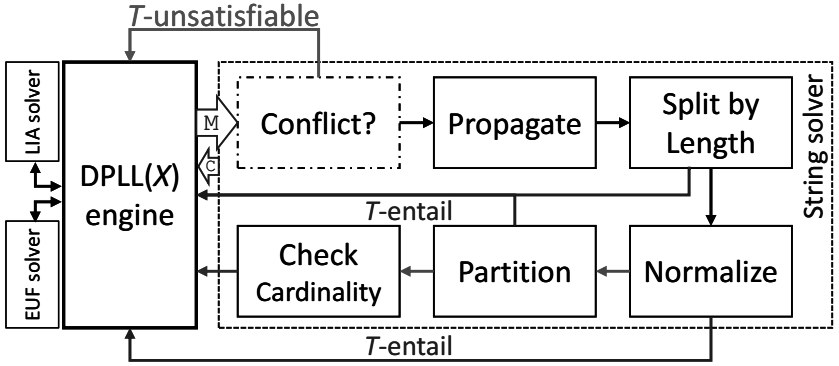
\includegraphics[width=0.7\linewidth]{pictures/proof_procedure.png}
	\caption{Abstracted core proof procedure for string. The figure is taken from \cite{main_phd}.}
	\label{fig:proof_procedure}
	\end{figure}
	
	
	In this section, we will see how the derivation rules are applied to produce the derivation tree. According to the authors of paper \cite{main-paper} this proof procedure is a highly abstracted version of the one which is implemented in cvc4 string solver. The main procedure is based on the repeated application of the rules according to the seven steps below (also as shown in Figure \ref{fig:proof_procedure}). In cases of split, the left branch configuration is tried first. The procedure interrupts and restarts with Step 0 as soon as new constraint is introduced to $S$. The procedure keeps cycling through the steps until it derives a configuration where no rules applies or the \texttt{unsat} one. In the case of \texttt{unsat}, if there is other branch configuration, the procedure continues with that branch in the derivation tree.

\begin{description}			
	\item$Step\ 0:$ $Reset:$ Apply \texttt{Reset} to reset buckets, and flat and normal forms.
	\item$Step\ 1:$ $Check\ for\ conflicts:$ Apply \texttt{S-Conflict} or \texttt{A-Conflict} if the configuration is unsatisfiable due to the current string or arithmetic constraints.
	\item$Step\ 2:$ $Propagate:$ Apply \texttt{S-Prop} and \texttt{A-Prop} and propagate entailed equalities between $S$ and $A$.
	\item$Step\ 3:$  $Add\ length\ constraints:$ For each non-variable $t \in \mathcal{T}(S)$, apply \texttt{Len} to add the equality $ \texttt{len}(x)\approx \texttt{len}(t)$ to \texttt{A}.  For each variable $x$ in $\mathcal{V}(S \cup A)$, apply \texttt{Len-Split},and then first explore the branch where $x \approx \epsilon$.
	\item$Step\ 4:$ $Compute\ Normal\ Forms\ for\ Equivalence\ Classes:$ Apply \texttt{S-Cycle} to shrinks concatenation terms. Then apply the normalization rules \texttt{F-Form1},\texttt{F-Form2}, \texttt{N-Form1} and \texttt{N-Form2} to completion. The idea is to produce a total map $N$. If not, then rules like \texttt{L-Split}, \texttt{F-Unify}, \texttt{F-Split}, \texttt{F-loop} are applied according to different cases. Detail on this can be found on paper \cite{main_phd}.
		
	\item$Step\ 5: Partition\ equivalence\ classes\ into\ buckets:$ The target is to distribute each equivalence class to a bucket. First apply \texttt{D-Base} and \texttt{D-Add} to completion. This should make $B$ a partition of \( \textnormal{E}_S \). If not, then there is an equivalence class $[x]$ which is not contained in any bucket. At this step rules like \texttt{S-Split}, \texttt{D-Split}, \texttt{L-Split} are applied according to different cases. Detail on this can be found on paper \cite{main_phd}.
	\item$Step\ 6:Add\ length\ constraint\ for\ cardinality:$ Apply the rule \texttt{Card} for each bucket. This will introduce new arithmetic constraints corresponding to the minimal length of terms in $B$ based on the number of equivalence classes in $B$ and the cardinality $| \mathcal{A}|$ of the alphabet. For instance, if $\Sigma$ is a finite alphabet of 256 characters and $S$ entails that 257 distinct strings of length 1 exist, then $S$ is unsatisfiable. 
\end{description}
    In this section, we have presented a brief and abstract overview of the procedure. The description of the different steps are taken from \cite{main_phd}. In the subsequent section we will present few examples of the application of the derivation according to this procedure.

    \subsection{Examples}
Now we try to illustrate the procedure's workings with respect of two example. First example shows how the procedure conclude $unsat$ for a set of constraints which are unsatisfiable. And the second shows how the procedure finds a saturated configuration for a set of constraints which are satisfiable. Both the examples are taken from \cite{main-paper}.
\begin{description}			
	\item[Example 1:] The input constraints are: $ A = \phi$ and $S = \{ \texttt{len}(x) \approx
	\texttt{len}(y), x \not\approx \epsilon, y\not\approx \epsilon, z \not\approx \epsilon, \texttt{con}(x, l_1, z) \approx \texttt{con}(y, l_2, z)\}$, where $l_1$, $l_2$ are distinct constants of the same length.	

The procedure starts with $step\ 0$ by applying \texttt{Reset}. It tries to find conflicts by applying   \texttt{S-Conflict} and \texttt{A-Conflict}. Since the arithmetic constraint set $A$ is empty and there are no contradicting string constraints in $S$, $check\ for\ contradiction$ fails. 

The procedure tries the step $propagate$. For this example this step does not introduce any new constraint in $S$, as $A$ is empty. Now the procedure applies \texttt{Len} and \texttt{Len-Split} repeatedly as long as there is possible application. The application of these two splitting rules causes the branching of the derivation tree. However, all branches are closed by rule  \texttt{S-Conflict} expect one. This is shows in Figure as the left branches of each configuration. 

In this non closing configuration, the string equivalence classes are $\{x\}, \{y\}, \{z\}, \{l_1\}, \{l_2\}, \{\epsilon\},$ and $\{ \texttt{con}(x, l_1, z), \texttt{con}(y, l_2, z)\}$. Now the procedure goes on to compute normal forms by applying \texttt{N-Form2}, \texttt{F-Form2} and \texttt{N-Form1}.The flat forms  \texttt{F} $\texttt{con}(x, l_1, z) = (x, l_1, z)$ and \texttt{F} $\texttt{con}(y, l_2, z) = (y, l_2, z)$ are computed by \texttt{F-Form1}. Then \texttt{F-Unify} is applied to add the equality $x \approx y$ to $S$. This causes the procedure to restart, but with an extended constraints set. Which induces a new equivalence classes $ \{x, y\}, \{z\}, \{l_1\}, \{l_2\}, \{\epsilon\}$, and $\{\texttt{con}(x, l_1, z), \texttt{con}(y, l_2, z)\}$. After similar steps, the procedure reached a stage where it computes the flat forms $(x, l_1, z)$ and $(x, l_2, z)$ for the  corresponding equivalence class,
by choosing $x$ as representative of $y$. At this point the procedure applies rule \texttt{F-Unify} again. This introduces a new equality $l_1 \approx l_2$ to $S$ and eventually derives \texttt{unsat} with \texttt{S-Conflict}. That is the procedure ended up with a derivation tree where each branch is closed and conclude that the input constraints are unsatisfiable.  The resulting derivation tree is shown in figure .

\begin{figure}
	\centering
	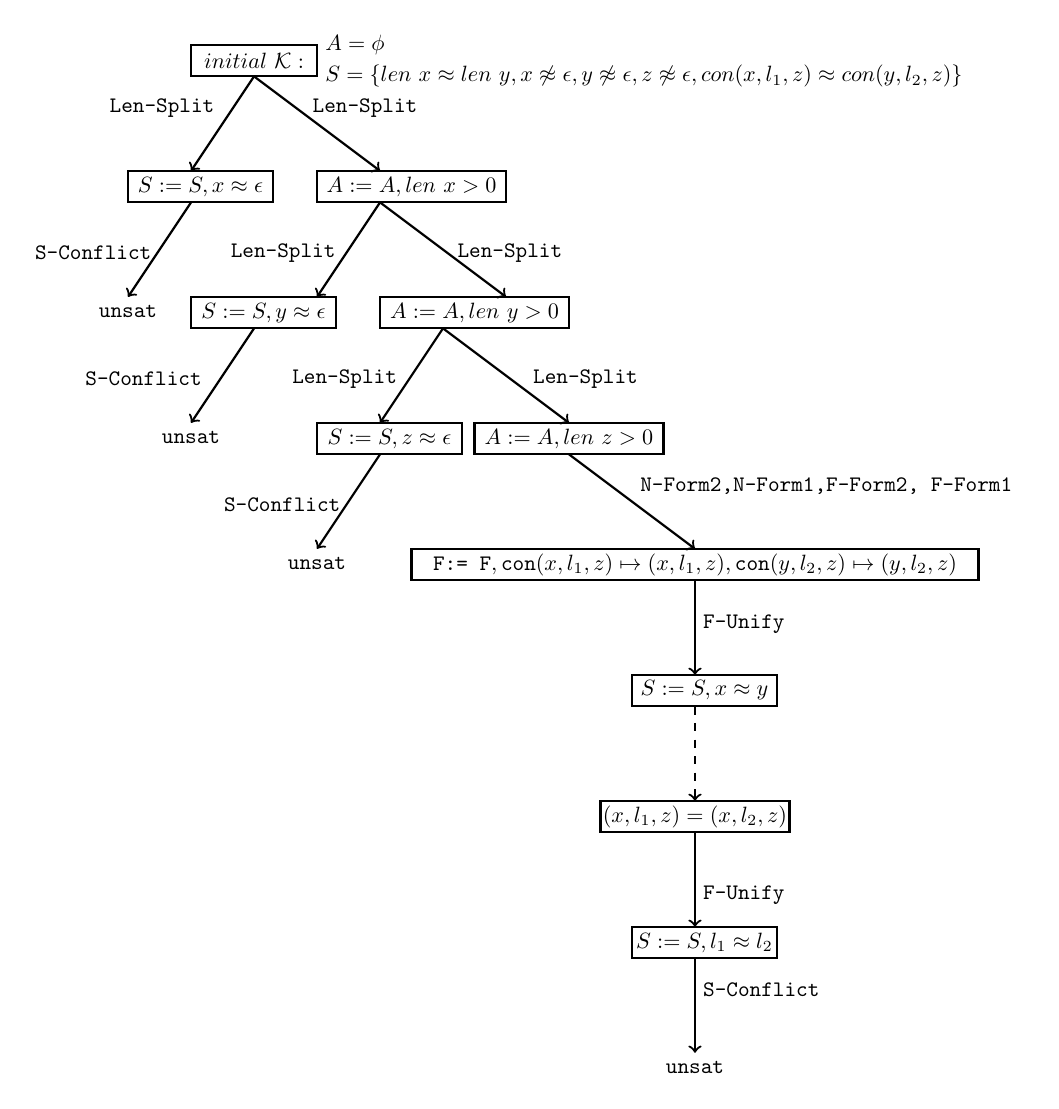
\begin{tikzpicture}[thick,scale=0.8, every node/.style={transform shape}]
	
	\node [right] at (3,20) { $ A=\phi $};
	\node [right] at (3,19.5) { $ S=\{  len \ x \approx len \ y, x \not\approx \epsilon, y \not\approx \epsilon,
		z \not\approx \epsilon, con (x, l_1,z) \approx con (y, l_2, z)\} $}; 
	 
    \draw (1,20) rectangle (3,19.5) node[pos=.5] {$ initial \ \mathcal{K}:$};
	
	\draw [->] (2,19.5) -- (1,18);
	\node [left] at (1.5,19) {$\texttt{Len-Split}$};
	
	\draw [->] (2,19.5) -- (4,18);
	\node [right] at (2.8,19) {$\texttt{Len-Split}$};
	
	
	\draw (0,18) rectangle (2.3,17.5) node[pos=.5] {$S:=S, x\approx \epsilon$};
	\node [rectangle, below] at (1,18) {};
	
	
	\draw (3,18) rectangle (6,17.5) node[pos=.5] {$A:=A, len \ x  > 0$};
	\node [rectangle, below] at (4,18) {};
	
	\draw [->] (1,17.5) -- (0,16);
	\node [left] at (0.5,16.7) {$\texttt{S-Conflict}$};
	
	\draw [->] (4,17.5) -- (3,16);
	\node [right] at (1.5,16.7) {$\texttt{Len-Split}$};
	\draw [->] (4,17.5) -- (6,16);
	\node [right] at (5.1,16.7) {$\texttt{Len-Split}$};
	
	\node [below] at (0,16) {$\texttt{unsat}$};
	\draw (1,16) rectangle (3.3,15.5) node[pos=.5] {$S:=S, y\approx \epsilon$};
	\node [below] at (2,16) {};
	\draw (4,16) rectangle (7,15.5) node[pos=.5] {$A:=A, len \ y  > 0$};
	\node [below] at (5,16) {};
	
	\draw [->] (2,15.5) -- (1,14);
	\node [left] at (1.3,14.7) {$\texttt{S-Conflict}$};
	\draw [->] (5,15.5) -- (4,14);
	\node [left] at (4.4,14.7) {$\texttt{Len-Split}$};	
	\draw [->] (5,15.5) -- (7,14);
	\node [right] at (6.3,14.7) {$\texttt{Len-Split}$};
	
	
	\node [below] at (1,14) {$\texttt{unsat}$};
	\draw (3,14) rectangle (5.3,13.5) node[pos=.5] {$S:=S, z\approx \epsilon$};
	\node [below] at (4,14) {};
	\draw (5.5,14) rectangle (8.5,13.5) node[pos=.5] {$A:=A, len \ z  > 0$};
	\node [below] at (7,14) {};


	\draw [->] (4,13.5) -- (3,12);
	\node [left] at (3.5,12.7) {$\texttt{S-Conflict}$};
	\draw [->] (7,13.5) -- (9,12);
    \node [right] at (8,13) {$\texttt{N-Form2,N-Form1,F-Form2, F-Form1 }$};
    

	
	\node [below] at (3,12) {$\texttt{unsat}$};
	\draw (4.5,12) rectangle (13.5,11.5) node[pos=.5] {$\texttt{F:= F},\texttt{con}(x,l_1,z)\mapsto (x,l_1,z),\texttt{con}(y,l_2,z)\mapsto(y,l_2,z)$};
	\node [below] at (9,12) {};
	
	\draw [->] (9,11.5) -- (9,10);
	\node [right] at (9,10.8) {$\texttt{F-Unify}$};
	
	\draw (8,10) rectangle (10.3,9.5) node[pos=.5] {$S:=S, x\approx y$};
	\node [below] at (9,10) {};
	
	\draw [dashed,->] (9,9.5) -- (9,8);
	
	\draw (7.5,8) rectangle (10.5,7.5) node[pos=.5] {$( x, l_1, z ) = (x, l_2,z)$};
	\node [below] at (9,8) {};
	
	\draw [->] (9,7.5) -- (9,6);
	\node [right] at (9,6.5) {$\texttt{F-Unify}$};
	
	\draw (8,6) rectangle (10.3,5.5) node[pos=.5] {$S:=S, l_1 \approx l_2$};
	\node [below] at (9,6) {};
	
	\draw [->] (9,5.5) -- (9,4);
	\node [right] at (9,5) {$\texttt{S-Conflict}$};
	
	\node [below] at (9,4) {$\texttt{unsat}$};
	
	
	
	
	
	
	\end{tikzpicture}
	\caption{The derivation tree for example 1. Here $l_1, l_2 $ are distinct constants of same length.}
\end{figure}	


	
	
\end{description}
\begin{description}			
	\item[Example 2:] The input constraints are: $ A = \phi$ and $S = \{ \texttt{len}(x) \approx
	\texttt{len}(y), x \not\approx \epsilon, z \not\approx \epsilon, \texttt{con}(x, l_1, z) \not\approx \texttt{con}(y, l_2, z)\}$, with $l_1$, $l_2$ are distinct constants of the same length.
	
	
	Similar to the previous example, the procedure reaches a configuration where the string equivalence classes are $ \{x\}, \{y\}, \{z\}, \{l_1\}, \{l_2\}, \{\epsilon\},\{ \texttt{con}(x, l_1, z)\}$ and,$\{\texttt{con}(y, l_2, z)\}$.
	In this case, the procedure attempts to partition the the equivalence classes into buckets. It fails to create the full partition, as rule \texttt{D-Base}  nor rule \texttt{D-Add} is applicable to $[y]$ because of $S \models \texttt{len} \ x \approx \texttt{len} \ y$ and  $x \not\approx y \not\in \mathcal{C}(S)$.  
	
	In such a case the procedure tries to guess by applying rule \texttt{S-Split} to $x$ and $y$. It case two branches in the derivation tree, one for $x \approx y$ and another for $x \not\approx y$.  
		
	After similar steps as in previous example, the procedure can derive a configuration where the string equivalence classes are $ \{x\}, \{y\}, \{z\}, \{l_1\}, \{l_2\}, \{\epsilon\},\{ \texttt{con}(x, l_1, z)\}$ and,$\{\texttt{con}(y, l_2, z)\}$. After computing normal forms for these classes, it attempts to	construct a partition \texttt{B} of them into buckets. However, notice that if it adds {[x]},say, to \texttt{B} using \texttt{D-Base}, then neither \texttt{D-Base} (since $S \models \texttt{len} \ x \approx \texttt{len} \ y$) nor \texttt{D-Add} (since $x \not\approx y \not\in \mathcal{C}(S)$ ) is applicable to $[y]$. So it applies \texttt{S-Split} to $x$ and $y$. In the branch where $ x \approx y$, the procedure subsequently restarts as new constraints are introduced to $S$. Eventually the procedure computes normal forms and succeeds in making a full partition of \texttt{B}. The procedure places $[\texttt{con}(x, l_1, z)]$ and $[\texttt{con}(y, l_2, z)]$ into the same bucket using \texttt{D-Add}, which applies because their corresponding normal forms are $(x, l_1, z)$ and $(x, l_2, z)$ respectively. Any further rule applications lead to branches with  a saturated configuration. Thus the procedure concludes that the problem is satisfiable. For each of the branches with saturated configuration satisfying models can be generated.
\end{description}
Here in this section we have tried to explore the inner working of the decision procedure. According to the authors \cite{main-paper}, the presented version the procedure is a simplified one. The procedure and derivation rules, which are implemented as part of cvc4 is much more complex and elaborate.
    \subsection{Integration  into SMT solver architecture}
\label{sec:Implementation in DPLLt}
In this section we will explain, how the string theory solver is integrated into modern DPLL($T$) framework.
We will briefly discuss the issues of $theory\ propagation$, $lemma\ learning$ and $conflict\ analysis$.

 
Modern SMT solvers combine a SAT solver with multiple specialized $theory\ solvers$. The SAT solver maintain an evolving set $F$ of clauses and a set $M$ of literals representing partial assignment. The whole process is derived by the SAT solver. It periodically consults the theory solver, to find whether $M$ is satisfiable in its theory. The literals of an assignment $M$ are partitioned into string constraints, arithmetic constraints. These sets are subsequently given to the independent solvers. The rules \texttt{A-Prop} and \texttt{S-Prop} model the mechanism for $theory\ combination$. This mechanism is known as Nelson-Oppen theory combination \cite{nelson_oppen}, where the entailed equalities are communicated between multiple solvers. The rule \texttt{A-Conflict} modeled the satisfiability checking done by the arithmetic solver. As there is no additional requirement for the arithmetic solver, a standard theory solver for linear integer arithmetic can be used. 

The case splitting done by the string solver (with rules \texttt{S-Split} and \texttt{L-Split}) is achieved by means of the $splitting\ on\ demand$ paradigm, in which a solver may add theory lemmas to $F$ consisting of clauses possibly with literals not occurring in $M$.  This approach of $lemma\ learning$ is very efficient as new lemmas are introduced only when it is needed.  Similarly, the rules \texttt{Len}, \texttt{Len-Split}, and \texttt{Card} are involved in introduction of new constraints into \texttt{A}. This is done by the string solver by adding lemmas to ${F}$ containing arithmetic constraints. For example, if $x \approx \texttt{con}(y, z) \in \mathcal{C}(\texttt{S})$, the solver may add a lemma of the form $ \psi \Rightarrow \texttt{len}\ x \approx \texttt{len}\ y + \texttt{len}\ z$ to $F$, where $\psi$ is a conjunction of literals from $M$ entailing $x \approx \texttt{con}(y, z)$, after which the conclusion of this lemma is added to $M$.

When a theory solver determines that $M$ is unsatisfiable, it produces a $conflict\ clause$ to support the decision. A $conflict\ clause$ is the negation of an unsatisfiable subset of $M$. Whenever the string solver introduces any equality to \texttt{S}, it also maintains an explanation $ \psi_{s,t}$ for each equality $s \approx t$. An explanation $\psi_{s,t}$ is a conjunction of string constraints in $M$ such that $\psi_{s,t} \models s \approx t$. When a configuration is decided to be unsatisfiable by rule \texttt{S-Conflict},that is, when $ s \approx t, s \not\approx t \in \mathcal{C}(\texttt{S})$ for some $s, t,$ it replaces the occurrence of $s \approx t$ with its corresponding explanation $\psi$, and then replaces the equalities in $\psi$ with their corresponding explanation, and so on, until $\psi$ contains only equalities from $M$. Finally, it reports the conflict clause 
$ \psi \Rightarrow s \approx t$.

The core idea of the above explanations are taken from \cite{main-paper}.
    \section{Correctness}
\label{sec:Correctness}
The procedure is $refutation\ sound$, that is when the procedure answers \texttt{unsat}, it can be trusted even for strings of unbounded length. And the procedure is $solution\ sound$, that is when the procedure answers $sat$, it can be trusted. In the original paper \cite{main-paper}, the authors have claimed that they have a version of the procedure which is also $solution\ complete$, that is when the procedure answers $sat$, it will eventually get a model by finite model finding. However, the procedure  is $refutation\ complete$, that is for an unsatisfiable set of constraints the procedure may not terminate. More detail on the correctness properties and the proofs of these theorem can be found in \cite{main_phd}.
    
    
    
    %\begin{figure}
	\centering
	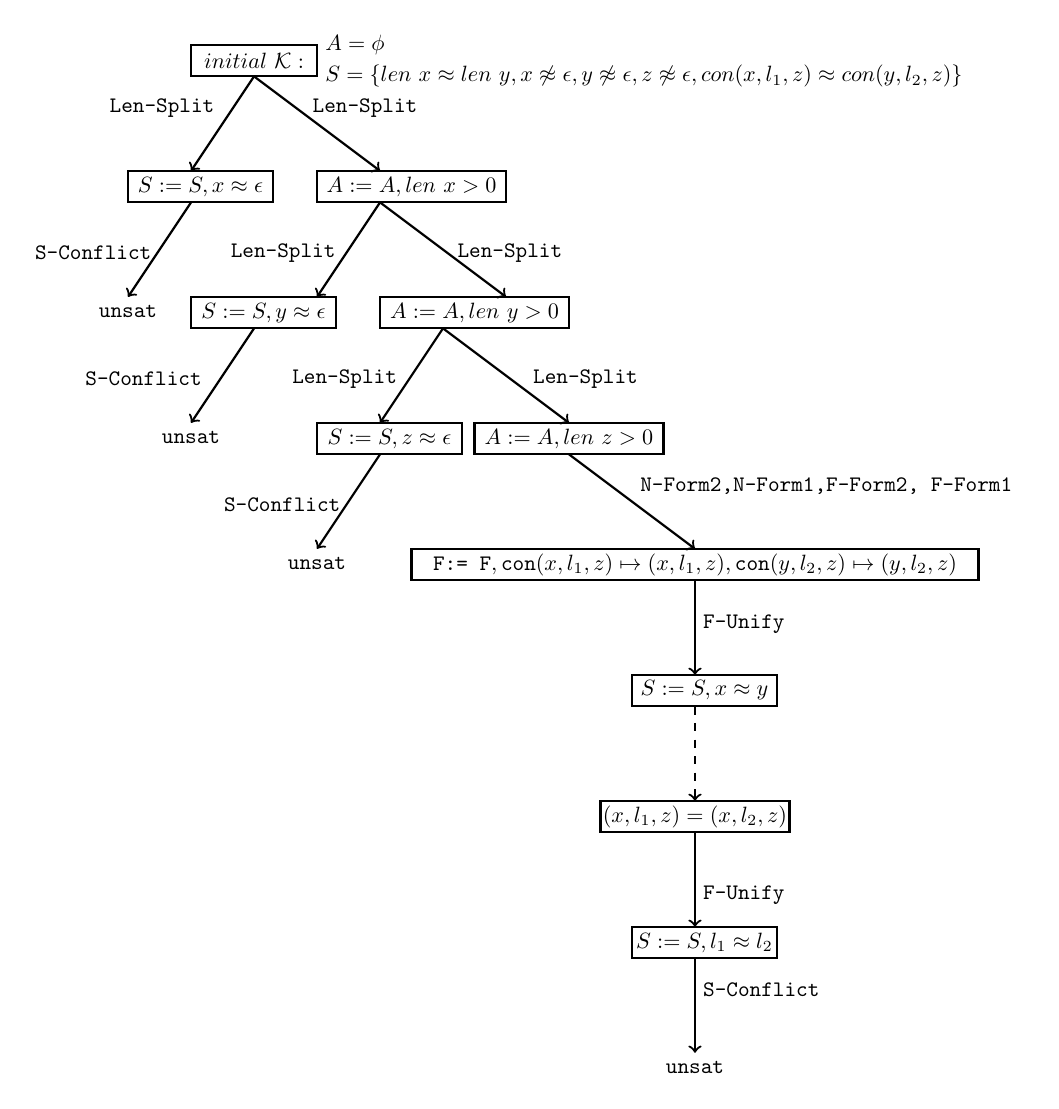
\begin{tikzpicture}[thick,scale=0.8, every node/.style={transform shape}]
	
	\node [right] at (3,20) { $ A=\phi $};
	\node [right] at (3,19.5) { $ S=\{  len \ x \approx len \ y, x \not\approx \epsilon, y \not\approx \epsilon,
		z \not\approx \epsilon, con (x, l_1,z) \approx con (y, l_2, z)\} $}; 
	 
    \draw (1,20) rectangle (3,19.5) node[pos=.5] {$ initial \ \mathcal{K}:$};
	
	\draw [->] (2,19.5) -- (1,18);
	\node [left] at (1.5,19) {$\texttt{Len-Split}$};
	
	\draw [->] (2,19.5) -- (4,18);
	\node [right] at (2.8,19) {$\texttt{Len-Split}$};
	
	
	\draw (0,18) rectangle (2.3,17.5) node[pos=.5] {$S:=S, x\approx \epsilon$};
	\node [rectangle, below] at (1,18) {};
	
	
	\draw (3,18) rectangle (6,17.5) node[pos=.5] {$A:=A, len \ x  > 0$};
	\node [rectangle, below] at (4,18) {};
	
	\draw [->] (1,17.5) -- (0,16);
	\node [left] at (0.5,16.7) {$\texttt{S-Conflict}$};
	
	\draw [->] (4,17.5) -- (3,16);
	\node [right] at (1.5,16.7) {$\texttt{Len-Split}$};
	\draw [->] (4,17.5) -- (6,16);
	\node [right] at (5.1,16.7) {$\texttt{Len-Split}$};
	
	\node [below] at (0,16) {$\texttt{unsat}$};
	\draw (1,16) rectangle (3.3,15.5) node[pos=.5] {$S:=S, y\approx \epsilon$};
	\node [below] at (2,16) {};
	\draw (4,16) rectangle (7,15.5) node[pos=.5] {$A:=A, len \ y  > 0$};
	\node [below] at (5,16) {};
	
	\draw [->] (2,15.5) -- (1,14);
	\node [left] at (1.3,14.7) {$\texttt{S-Conflict}$};
	\draw [->] (5,15.5) -- (4,14);
	\node [left] at (4.4,14.7) {$\texttt{Len-Split}$};	
	\draw [->] (5,15.5) -- (7,14);
	\node [right] at (6.3,14.7) {$\texttt{Len-Split}$};
	
	
	\node [below] at (1,14) {$\texttt{unsat}$};
	\draw (3,14) rectangle (5.3,13.5) node[pos=.5] {$S:=S, z\approx \epsilon$};
	\node [below] at (4,14) {};
	\draw (5.5,14) rectangle (8.5,13.5) node[pos=.5] {$A:=A, len \ z  > 0$};
	\node [below] at (7,14) {};


	\draw [->] (4,13.5) -- (3,12);
	\node [left] at (3.5,12.7) {$\texttt{S-Conflict}$};
	\draw [->] (7,13.5) -- (9,12);
    \node [right] at (8,13) {$\texttt{N-Form2,N-Form1,F-Form2, F-Form1 }$};
    

	
	\node [below] at (3,12) {$\texttt{unsat}$};
	\draw (4.5,12) rectangle (13.5,11.5) node[pos=.5] {$\texttt{F:= F},\texttt{con}(x,l_1,z)\mapsto (x,l_1,z),\texttt{con}(y,l_2,z)\mapsto(y,l_2,z)$};
	\node [below] at (9,12) {};
	
	\draw [->] (9,11.5) -- (9,10);
	\node [right] at (9,10.8) {$\texttt{F-Unify}$};
	
	\draw (8,10) rectangle (10.3,9.5) node[pos=.5] {$S:=S, x\approx y$};
	\node [below] at (9,10) {};
	
	\draw [dashed,->] (9,9.5) -- (9,8);
	
	\draw (7.5,8) rectangle (10.5,7.5) node[pos=.5] {$( x, l_1, z ) = (x, l_2,z)$};
	\node [below] at (9,8) {};
	
	\draw [->] (9,7.5) -- (9,6);
	\node [right] at (9,6.5) {$\texttt{F-Unify}$};
	
	\draw (8,6) rectangle (10.3,5.5) node[pos=.5] {$S:=S, l_1 \approx l_2$};
	\node [below] at (9,6) {};
	
	\draw [->] (9,5.5) -- (9,4);
	\node [right] at (9,5) {$\texttt{S-Conflict}$};
	
	\node [below] at (9,4) {$\texttt{unsat}$};
	
	
	
	
	
	
	\end{tikzpicture}
	\caption{The derivation tree for example 1. Here $l_1, l_2 $ are distinct constants of same length.}
\end{figure}	

    %\begin{figure}
\centering
\begin{tikzpicture}
\draw [lightgray](0,0) --(0,20) -- (15,20)-- (15,0) --(0,0);
\draw [lightgray](0,1) --(15,1);
\draw [lightgray](0,2) --(15,2);
\draw [lightgray](0,3) --(15,3);
\draw [lightgray](0,4) --(15,4);
\draw [lightgray](0,5) --(15,5);
\draw [lightgray](0,6) --(15,6);
\draw [lightgray](0,7) --(15,7);
\draw [lightgray](0,8) --(15,8);
\draw [lightgray](0,9) --(15,9);
\draw [lightgray](0,10) --(15,10);
\draw [lightgray](0,11) --(15,11);
\draw [lightgray](0,12) --(15,12);
\draw [lightgray](0,13) --(15,13);
\draw [lightgray](0,14) --(15,14);
\draw [lightgray](0,15) --(15,15);
\draw [lightgray](0,16) --(15,16);
\draw [lightgray](0,17) --(15,17);
\draw [lightgray](0,18) --(15,18);
\draw [lightgray](0,19) --(15,19);
\draw [lightgray](0,20) --(15,20);

\draw [lightgray](0,7.5) --(7.5,20);

\node [below] at (10,10) {$ initial \ \mathcal{K}$};
\node [below] at (10,9.6) {$\texttt{Len-Split}$};

\draw [->] (10,9.3) -- (8,8.5);
\draw [->] (10,9.3) -- (12,8.5);


\draw [->] (5,5) -- (4,4.5);
\node [right] at (2,8) {$\texttt{F:= F},\texttt{con}(x,l_1,z)\mapsto (x,l_1,z),\texttt{con}(y,l_2,z)\mapsto(y,l_2,z)$};
\node [right] at (6,7.2) {$\texttt{F-Unify}$};
\draw [->] (6,7.8) -- (6,6.8);
\node [right] at (5,6.5) {$\texttt{S:= S},x\approx y$};

\end{tikzpicture}
\caption{The derivation tree for example 1.}
\end{figure}



    \section{Evaluation}
\label{sec:evaluation}
According to the authors \cite{main-paper}, a theory solver based procedure described in the previous sections, is implemented as part of SMT solver CVC4. The string alphabet $\mathcal{A}$ for this implementation is the set of all 256 ASCII characters. An experimental comparison with two other the string solvers was conducted. The other string solvers are Z3-STR \cite{Z3_str} and Kaluza \cite{Kaluza}. These two solvers are widely used in security analysis. For the evaluation, 47,284 benchmark problems from a set of about 50K benchmarks generated by Kudzu \cite{Kudzu} were used. These benchmarks were translated into CVC4’s extension of the SMT-LIB format and into the Z3-STR format. In the paper \cite{main-paper}, it is claimed that, CVC4’s string solver performed better. More detail on the evaluation can be found in \cite{main_phd}.
    \section{Conclusion}
\label{sec:conclusion}
In this paper, we tried to present the overview of a automatic reasoning tool for solving constraints over unbounded strings with length. We have found, the idea of implementing the string solver natively is unique. This approach allowed high interaction with core of CVC4 SMT solver. So the performance is better than others. It also allows any general purpose arithmetic solver be easily integrated. However, the application of the rules is complicated and very hard to implement. it would be better to support a richer language of string constraints that occur often in practice, especially in security applications. Such expressiveness would promote the use of such automatic reasoning tool in commercial software constructions. 
    
	
	\newpage
	%Sets the bibliography style to UNSRT and imports the 
	%bibliography file "samples.bib".
	\bibliographystyle{unsrt}
	\bibliography{sample}
	
\end{document}

